% Theorie: Physikalische Grundlagen von Versuch/Messverfahren, Gleichungen ohne Herleitung knapp erklären
\section[Theorie]{Theorie \textnormal{\cite{millikan}}}
\label{sec:theorie}

Die für den Versuch nach Millikan benötigten Öltröpfchen werden beim Zerstäuben durch gegenseitige Reibung elektrisch geladen. Da die getragene
Ladung immer einem ganzzahligen Vielfachen der Elementarladung $e_0$ entspricht, lässt sich diese bestimmen, indem die Tröpfchen in ein vertikales
elektrisches Feld gebracht werden. Dieses wird näherungsweise homogen zwischen zwei Kondensatorplatten realisiert und erlaubt nach
Aufstellen eines Kräftegleichgewichts die Berechnung der Ladung.

\begin{figure}[H]
	\centering
	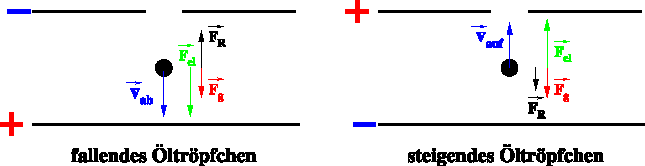
\includegraphics[width=0.75\linewidth]{content/grafik/gleichgewicht.pdf}
	\captionsetup{width=0.925\linewidth}
	\caption{Vektordiagramm der auf ein Öltröpfchen wirkenden Kräfte im homogenen elektrischen Feld unter Berücksichtigung der Polung.}
	\label{fig:gleichgewicht}
\end{figure}

Ein Tröpfchen mit Masse $m$ und Dichte $\rho_O$ erfährt die Gravitationskraft $\symbf F_G = m \symbf g$ und wird entsprechend nach unten
beschleunigt. Entgegen der Bewegungsrichtung wirkt mit $\symbf F_R = -6\pi r \eta_L \symbf v$ die Stokessche Reibungskraft, wobei $\eta_L$
die Viskosität der Luft sowie $r$ den Radius und $\symbf v$ die Geschwindigkeit des Öltröpfchens bezeichnen. Der Vollständikeit halber soll
hier auch der Auftrieb $\symbf F_{\! A}$ in Luft berücksichtigt werden, obwohl sein Beitrag wegen der geringen Dichte verschwindend gering ausfällt.
Werden die Tropfen als kugelförmig angenommen, ergibt sich ihre Masse zu
\begin{equation*}
	m = \rho_O V = \pfrac{4}{3} \pi r^3 \rho_O \: .
\end{equation*}
Nach kurzzeitiger Beschleunigungsphase stellt sich ein Kräftegleichgewicht mit passender Gleichgewichtsgeschwindigkeit $\symbf v_0$ ein.
Es gilt also
\begin{equation*}
	\symbf F_G = \symbf F_R + \symbf F_{\! A} \: .
\end{equation*}
Entspricht $\rho_L$ der Dichte des umgebenden Gasgemisches, liefert Einsetzen der Beträge und anschließendes Umstellen den Ausdruck
\begin{equation}
	\pfrac{4}{3} \pi r^3 \left( \rho_O - \rho_L \right) g = 6\pi \eta_L r v_0 \: .
	\label{eqn:gleichgewicht}
\end{equation}

Daraus lässt sich der Tröpfchenradius abhängig von sekundären Messgrößen über
\begin{equation}
	r = \sqrt{ \pfrac{9 \eta_L v_0}{2g \left( \rho_O - \rho_L \right)} }
	\tag{2a}
	\label{eqn:radius_a}
\end{equation}
darstellen. Nun wird der Einfluss $\symbf F_C = q \symbf E$ des elektrischen Feldes auf eine Ladung $q$ im Plattenkondensator betrachtet.
Ist dazu die Polung wie links in Abbildung~\ref{fig:gleichgewicht} angelegt, steht $\symbf F_C$ parallel zu $\symbf F_G$ gerichtet,
aus \eqref{eqn:gleichgewicht} folgt dann
\begin{align*}
	\pfrac{4}{3} \pi r^3 \left( \rho_O - \rho_L \right) g - 6\pi \eta_L r v_\text{ab} &= -q E \: . \\
	\intertext{Hier gibt $E$ die Feldstärke und $v_\text{ab}$ die gleichförmige Sinkgeschwindigkeit an. Wird das elektrostatische Feld in
		entgegengesetzter Anordnung bei ausreichend großen Stärken betrieben, führt das Öltröpfchen eine Aufwärtsbewegung mit
		Geschwindigkeit $v_\text{auf}$ aus, sodass nach \eqref{eqn:gleichgewicht} der Term}
	\pfrac{4}{3} \pi r^3 \left( \rho_O - \rho_L \right) g + 6\pi \eta_L r v_\text{auf} &= +q E
\end{align*}
formuliert werden kann. Wie rechts in Abbildung~\ref{fig:gleichgewicht} zu sehen ist, wechselt $\symbf F_R$ hier das Vorzeichen. Gleichsetzen
beider Fälle zu
\begin{equation*}
	\pfrac{4}{3} \pi r^3 \left( \rho_O - \rho_L \right) g - 6\pi \eta_L r v_\text{ab} =
	-\pfrac{4}{3} \pi r^3 \left( \rho_O - \rho_L \right) g - 6\pi \eta_L r v_\text{auf}
\end{equation*}
liefert durch die Umformung
\begin{equation*}
	\pfrac{8}{3} \pi r^3 \left( \rho_O - \rho_L \right) g = 6\pi \eta_L r \left( v_\text{ab} - v_\text{auf} \right)
\end{equation*}
eine alternative Darstellung für den Tropfenradius
\begin{equation}
	r = \sqrt{ \pfrac{9 \eta_L \left( v_\text{ab} - v_\text{auf} \right) }{4g \left( \rho_O - \rho_L \right)} } \: .
	\tag{2b}
	\stepcounter{equation}
	\label{eqn:radius_b}
\end{equation}
Anhand der Beziehungen \eqref{eqn:radius_a} und \eqref{eqn:radius_b} lässt sich die Forderung
\begin{equation}
	2 v_0 = v_\text{ab} - v_\text{auf}
	\label{eqn:bedingung}
\end{equation}
erkennen, welche zur Prüfung der Messgültigkeit herangezogen wird. Ist sie nicht erfüllt, kann davon ausgegangen werden, dass die Ladung $q$
des Öltröpfchens im Verlauf der Aufzeichnung variiert. Weiter kann $r$ in eine der zwei Gleichungen $\pm qE$ eingesetzt werden, sodass sich
die Ladung mit
\begin{equation}
	q = \pfrac{3\pi \eta_L}{\! E} \left( v_\text{ab} + v_\text{auf} \right)
	\sqrt{ \pfrac{9 \eta_L \left( v_\text{ab} - v_\text{auf} \right) }{4g \left( \rho_O - \rho_L \right)} }
	\label{eqn:ladung}
\end{equation}
beschreiben lässt. Es ist dann noch eine zusätzliche Einschränkung zu berücksichtigen:
\newpage
Das Gesetz von Stokes gilt nur für Tröpfchen, die eine Ausdehnung größer als die mittlere Weglänge $\bar{l}$ in Luft aufweisen. Da dies
für den betrachteten Versuch nicht gegeben ist, muss die Viskosität zu
\begin{equation}
	\hat{\eta}_L = \pfrac{\eta_L}{1 + \displaystyle{\pfrac{B}{\raisebox{1ex}{\( pr \)}}}}
	\label{eqn:viskos}
\end{equation}
korrigiert werden. Dabei findet der Cunningham-Korrekturterm $B = \qty{8.226e-3}{\pascal\meter}$ Verwendung, mit $p$ wird der
Luftdruck bezeichnet. Wegen $q \sim \eta_L^{3 / 2}$ folgt direkt
\begin{equation}
	\hat{q} = q \left( 1 + \displaystyle{\pfrac{B}{\raisebox{1ex}{\( pr \)}}} \right)^{\!\! - 3 / 2}
	\label{eqn:korrekt}
\end{equation}
als Vorschrift für die Korrektur der Ladung.

Nach Bestimmung der Elementarladung $e_0$ kann über die sogenannte Faraday-Konstante $F = \qty{9.649e4}{\coulomb\per\mole}$ 
die Avogadrokonstante $N_{\! A}$ leicht berechnet werden. Die Größe $F$ beschreibt die elektrische Ladung eines Mols einfach geladener Ionen,
daraus ergibt sich der Zusammenhang
\begin{equation}
	N_{\! A} = \pfrac{F}{\raisebox{0.75ex}{\( e_0 \)}} \: .
	\label{eqn:faraday}
\end{equation}

